\tikzset{>=latex} % for LaTeX arrow head

\colorlet{myblue}{blue!20}
\colorlet{mydarkblue}{blue!50!black}
\colorlet{myred}{black!50!red}

\tikzset{
  cube/.pic={
    \tikzset{every edge quotes/.append style={midway,auto},/cube/.cd,#1}
    \def\csize{2*\cubesize}
    \draw [every edge/.append style={pic actions,densely dashed,opacity=.5},pic actions]
    (0,0,0) coordinate (o)
            edge coordinate [pos=1] (g) ++(0,0,-\csize)
        --++(0,\csize,0) coordinate (a)
        --++(\csize,0,0) coordinate (b)
        --++(0,-\csize,0) coordinate (c) -- cycle
    (a) --++(0,0,-\csize) coordinate (d) edge (g)
        --++(\csize,0,0) coordinate (e) -- (b) -- cycle
    (c) -- (b) -- (e)
        --++(0,-\csize,0) coordinate (f) edge (g) -- cycle;
    \path [every edge/.append style={pic actions, |-|}];
  },
  z={(-0.334,-0.334)},
  /cube/.search also={/tikz},
  /cube/.cd,
  size/.store in=\cubesize, size=1,
}

\tikzset{
  gasparticle/.pic={
    \tikzset{/gasparticle/.cd,#1}
    \draw[->,green!60!black] (0,0) -- (\vec);
    \node[circle,fill,inner sep=.8,fill=black!80!blue] at (0,0,0) {};
  }
  /gasparticle/.search also={/tikz},
  /gasparticle/.cd,
  vec/.store in=\vec, vec={90:0.5},
}

% GAS in a box



% GAS in a box - unpartioned


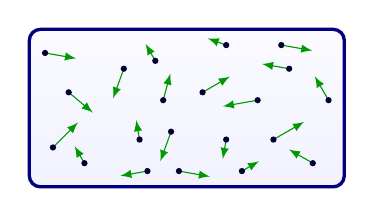
\begin{tikzpicture}
  \draw[mydarkblue,very thick,rounded corners=4,
        top color=blue!2,bottom color=blue!5,shading angle=0]
    (0,0) rectangle (4,2);
  \pic at (0.2,1.7) {gasparticle={vec={ -10:0.40}}};
  \pic at (0.3,0.5) {gasparticle={vec={  45:0.45}}};
  \pic at (0.5,1.2) {gasparticle={vec={ -40:0.40}}};
  \pic at (0.7,0.3) {gasparticle={vec={ 120:0.25}}};
  \pic at (1.2,1.5) {gasparticle={vec={-110:0.40}}};
  \pic at (1.4,0.6) {gasparticle={vec={ 100:0.25}}};
  \pic at (1.5,0.2) {gasparticle={vec={-170:0.35}}};
  \pic at (1.6,1.6) {gasparticle={vec={ 120:0.25}}};
  \pic at (1.7,1.1) {gasparticle={vec={  75:0.35}}};
  \pic at (1.8,0.7) {gasparticle={vec={-110:0.40}}};
  \pic at (1.9,0.2) {gasparticle={vec={ -10:0.40}}};
  \pic at (2.2,1.2) {gasparticle={vec={  30:0.40}}};
  \pic at (2.5,0.6) {gasparticle={vec={-100:0.25}}};
  \pic at (2.9,1.1) {gasparticle={vec={-170:0.45}}};
  \pic at (2.5,1.8) {gasparticle={vec={ 160:0.25}}};
  \pic at (2.7,0.2) {gasparticle={vec={  30:0.25}}};
  \pic at (3.1,0.6) {gasparticle={vec={  30:0.45}}};
  \pic at (3.2,1.8) {gasparticle={vec={ -10:0.40}}};
  \pic at (3.3,1.5) {gasparticle={vec={ 170:0.35}}};
  \pic at (3.6,0.3) {gasparticle={vec={ 150:0.35}}};
  \pic at (3.8,1.1) {gasparticle={vec={ 120:0.35}}};
\end{tikzpicture}
